\documentclass[convert={density=300,size=1080x800,outext=.png}]{standalone}
\usepackage{tkz-graph}
\usetikzlibrary{arrows,positioning,shapes,shapes.multipart,patterns,mindmap,shadows}
\usepackage{xcolor}
\usepackage{helvet}
\renewcommand{\familydefault}{\sfdefault}


\begin{document}

\footnotesize
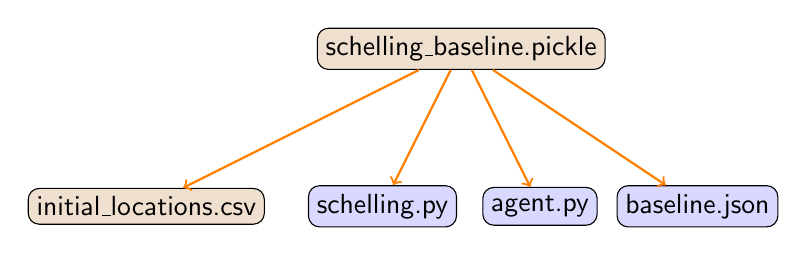
\begin{tikzpicture}[every node/.style={
    rectangle,
    rounded corners,
    inner sep=3pt,
    draw,
    fill=brown!25
}]
    \node (initial_locations_csv) [shift={(-4, 0)}]
    {
        initial\_locations.csv
    };
    \node (schelling_py) [fill=blue!15, shift={(-1, 0)}]
    {
        schelling.py
    };
    \node (agent_py) [fill=blue!15, shift={(1, 0)}]
    {
        agent.py
    };
    \node (baseline_json) [fill=blue!15, shift={(3, 0)}]
    {
        baseline.json
    };
    \node (schelling_baseline_pickle) [shift={(0, 2)}]
    {
        schelling\_baseline.pickle
    };
    \draw[->, orange, thick] (schelling_baseline_pickle) to (initial_locations_csv);
    \draw[->, orange, thick] (schelling_baseline_pickle) to (schelling_py);
    \draw[->, orange, thick] (schelling_baseline_pickle) to (agent_py);
    \draw[->, orange, thick] (schelling_baseline_pickle) to (baseline_json);
\end{tikzpicture}

\end{document}
